\documentclass[a4paper,twoside]{article}
\usepackage[T1]{fontenc}
\usepackage[bahasa]{babel}
\usepackage{graphicx}
\usepackage{graphics}
\usepackage{float}
\usepackage[cm]{fullpage}
\pagestyle{myheadings}
\usepackage{etoolbox}
\usepackage{setspace} 
\usepackage{lipsum} 
\setlength{\headsep}{30pt}
\usepackage[inner=2cm,outer=2.5cm,top=2.5cm,bottom=2cm]{geometry} %margin
% \pagestyle{empty}

\makeatletter
\renewcommand{\@maketitle} {\begin{center} {\LARGE \textbf{ \textsc{\@title}} \par} \bigskip {\large \textbf{\textsc{\@author}} }\end{center} }
\renewcommand{\thispagestyle}[1]{}
\markright{\textbf{\textsc{AIF401/AIF402 \textemdash Rencana Kerja Skripsi \textemdash Sem. Ganjil 2015/2016}}}

\onehalfspacing
 
\begin{document}

\title{\@judultopik}
\author{\nama \textendash \@npm} 

%tulis nama dan NPM anda di sini:
\newcommand{\nama}{Steven Sutana}
\newcommand{\@npm}{2012730046}
\newcommand{\@judultopik}{Porting PHP menjadi Play Framework (Studi Kasus : KIRI \textit{Front-End})} % Judul/topik anda
\newcommand{\jumpemb}{1} % Jumlah pembimbing, 1 atau 2
\newcommand{\tanggal}{26/08/2015} %%%%%%%%%%%%%%%%%%%%%%%%
\maketitle

\pagenumbering{arabic}

\section{Deskripsi}

\begin{center}
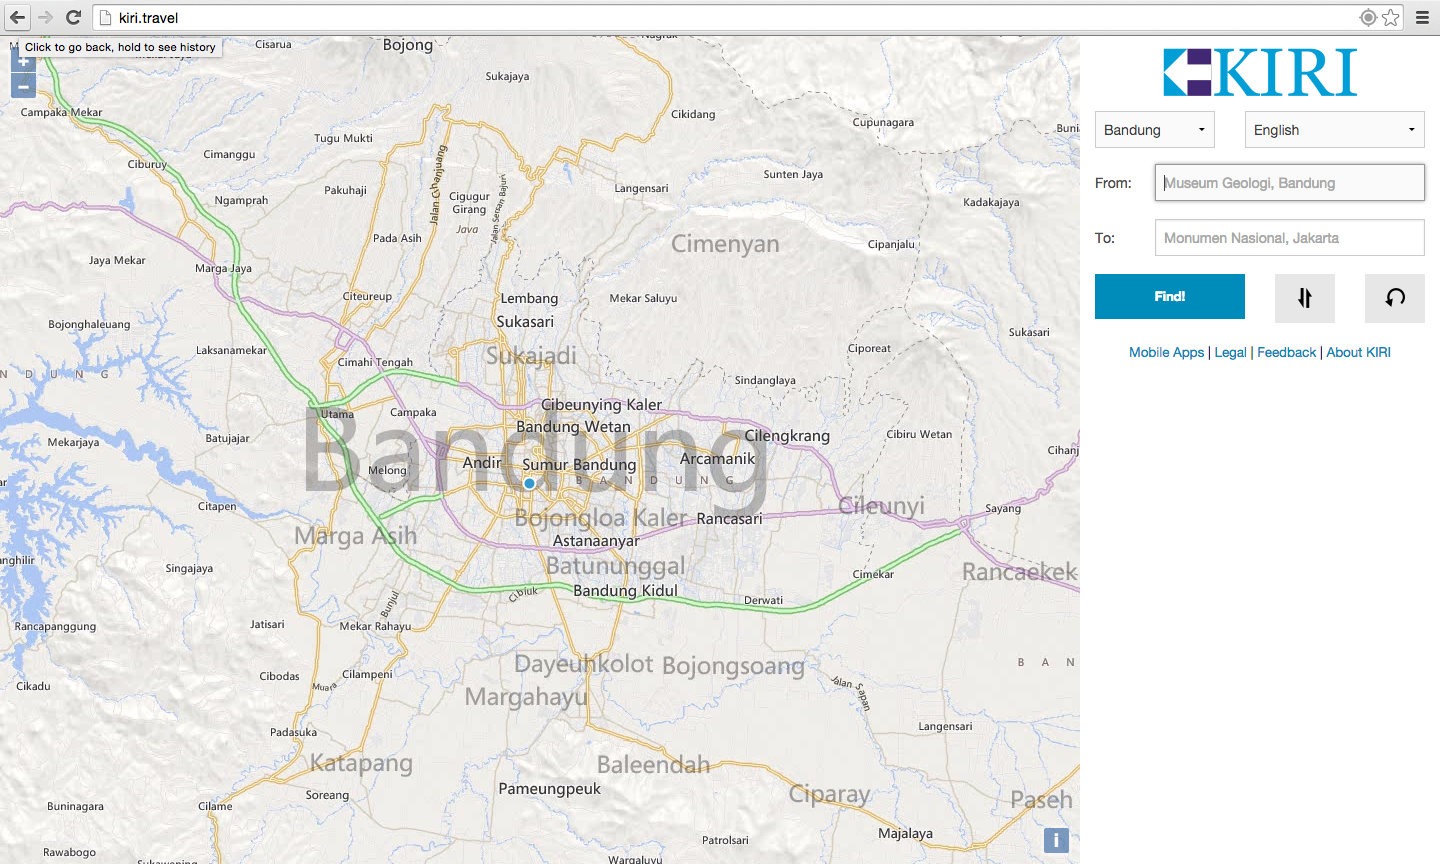
\includegraphics[scale = 0.3]{kiri.png}
\end{center}

KIRI (http://kiri.travel) merupakan aplikasi website yang membantu pengguna bepergian baik dalam kota maupun luar kota. Jika dalam kota, KIRI akan menentukan angkutan kota yang tersedia di kota tersebut, jika luar kota, maka KIRI menentukan travel yang tersedia ke kota yang akan dituju serta angkutan kota menuju tempat tujuan. Saat ini, KIRI tersedia dalam berbagai kota, yaitu Bandung, Depok, Jakarta, Surabaya, dan Malang. KIRI menyediakan berbagai rute alternatif yang dapat dipilih oleh pengguna. KIRI juga dapat membimbing pengguna langkah demi langkah untuk mencapai lokasi tujuan. 

Dalam pengembangan website, kita sering menjumpai bahasa yang dipakai adalah bahasa PHP. PHP tersebut kurang cocok dengan proyek besar. Masalah yang sering dijumpai seperti tidak ada deklarasi variabel, tidak ada tipe variabel. Dalam pengembangan website terdapat berbagai macam framework. Framework adalah kerangka yang membantu pengguna untuk menyelesaikan website. 

Dari berbagai framework yang dapat digunakan, dipilih Play Framework. Play Framework merupakan framework untuk membuat website dengan bahasa pemrograman Java. Play Framework menerapkan konsep MVC, yaitu Model, View, dan Controller. Dalam penelitian ini, Play Framework dipakai karena Play Framework terstruktur dan umum. 

\section{Rumusan Masalah}
\begin{itemize}
	\item Bagaimana memahami dan menganalisa kode KIRI yang sudah ada?
	\item Bagaimana melakukan porting kode KIRI (PHP) menjadi Play Framework (Java) ?
\end{itemize}

\section{Tujuan}
\begin{itemize}
	\item Memahami dan menganalisa kode KIRI.
	\item Menjadikan kode KIRI menjadi Play Framework.
\end{itemize}

\section{Deskripsi Perangkat Lunak}
Perangkat lunak akhir yang akan dibuat memiliki fitur minimal sebagai berikut:
\begin{itemize}
	\item Perangkat lunak dapat menampilkan tampilan KIRI secara terstruktur dengan menggunakan Play Framework.
	\item Perangkat lunak dapat berfungsi seperti website KIRI yang sudah ada sebagai \textit{Front-End Server Side}.
\end{itemize}

\section{Detail Pengerjaan Skripsi}
Bagian-bagian pekerjaan skripsi ini adalah sebagai berikut :
	\begin{enumerate}
		\item Memahami dan membedakan \textit{Front-End Server Side} dengan \textit{Front-End Client Side}
		\item Memahami dan melakukan analisa kode KIRI yang sudah ada.
		\item Melakukan studi literatur tentang metode yang berkaitan dengan kode PHP dan Java (Play Framework).
		\item Mempelajari cara kerja Play Framework untuk membuat website yang terstrtuktur.
		\item Merancang dan mengimplementasikan kode KIRI yang sudah ada menjadi Play Framework.
		\item Melakukan pengujian dan eksperimen.
		\item Membuat dokumen skripsi.
	\end{enumerate}

\section{Rencana Kerja}
\begin{center}
  \begin{tabular}{ | c | c | c | c | l |}
    \hline
    1*  & 2*(\%) & 3*(\%) & 4*(\%) &5*\\ \hline \hline
    1   & 5  & 5  &  &  \\ \hline
    2   & 5 & 5  &   & \\ \hline
    3   & 10  & 7  & 3 & {\footnotesize sebagian kecil teknik {\it flow tiles} di S2}  \\ \hline
    4   & 15  & 10  &  5 & {\footnotesize teknik lanjut OOP di C++ di S2} \\ \hline
    5   & 20  & 5  & 15 & {\footnotesize perancangan awal SFM, pathway dan waypoint di S1} \\ \hline
    6   & 5 &   & 5  & \\ \hline
    7   & 20  & 5  & 15 &  {\footnotesize implementasi denah dan rancangan awal SFM di S1}\\ \hline
    Total  & 100  & 40  & 60 &  \\ \hline
                          \end{tabular}
\end{center}

Keterangan (*)\\
1 : Bagian pengerjaan Skripsi (nomor disesuaikan dengan detail pengerjaan di bagian 5)\\
2 : Persentase total \\
3 : Persentase yang akan diselesaikan di Skripsi 1 \\
4 : Persentase yang akan diselesaikan di Skripsi 2 \\
5 : Penjelasan singkat apa yang dilakukan di S1 (Skripsi 1) atau S2 (skripsi 2)

\vspace{1cm}
\centering Bandung, \tanggal\\
\vspace{2cm} \nama \\ 
\vspace{1cm}

Menyetujui, \\
\ifdefstring{\jumpemb}{2}{
\vspace{1.5cm}
\begin{centering} Menyetujui,\\ \end{centering} \vspace{0.75cm}
\begin{minipage}[b]{0.45\linewidth}
% \centering Bandung, \makebox[0.5cm]{\hrulefill}/\makebox[0.5cm]{\hrulefill}/2013 \\
\vspace{2cm} Nama: \makebox[3cm]{\hrulefill}\\ Pembimbing Utama
\end{minipage} \hspace{0.5cm}
\begin{minipage}[b]{0.45\linewidth}
% \centering Bandung, \makebox[0.5cm]{\hrulefill}/\makebox[0.5cm]{\hrulefill}/2013\\
\vspace{2cm} Nama: \makebox[3cm]{\hrulefill}\\ Pembimbing Pendamping
\end{minipage}
\vspace{0.5cm}
}{
% \centering Bandung, \makebox[0.5cm]{\hrulefill}/\makebox[0.5cm]{\hrulefill}/2013\\
\vspace{2cm} Nama: \makebox[3cm]{\hrulefill}\\ Pembimbing Tunggal
}
`
\end{document}

